\documentclass[aspectratio=169]{beamer}
\usepackage[utf8]{inputenc}
\usepackage{microtype}
\usepackage{xspace}
\usepackage{scrextend}
\usepackage{listings}
\lstset{inputencoding=utf8,basicstyle=\ttfamily,backgroundcolor=\color{gray}}
\newcommand{\GR}{GNU\,Radio\xspace}
\usepackage{siunitx}
\sisetup{per-mode = fraction}
\DeclareSIUnit[number-unit-product = {\,}]\sample{S}
\usecolortheme[dark]{solarized}
\title {Getting your \texttt{perf}ormance up}
\logo{
\includegraphics[height=4em]{grcon}}
\author{Marcus Müller}
\institute{Ettus Research}
\date{September 16\textsuperscript{th} 2016}
\subtitle{Where did my cycles go?}
\usepackage{pgfplots}
\usepgfplotslibrary{fillbetween}
\begin{document}
\begin{frame}{}
  \titlepage
\mbox{\small Vaguely based on experience} 
\end{frame}
\begin{frame}
  \frametitle{Preface}
  \begin{itemize}
  \item The debugging: I'm stupid, but it's been a fun experience debugging
    this, kudos to noc0lour
  \item The Shell: This is \lstinline{zsh}, enhanced by \lstinline{oh-my-zsh},
    with the Hokietux-maintained \lstinline{Powerlevel9k} theme, running in
    \lstinline{gnome-terminal}, with a \lstinline{solarized-dark} color theme
    (which is the same used for this presentation)
    \item Shout if you spot mistakes. I'll repeat your heckle, so it's on
      record.
      \item funky animation: \url{https://github.com/marcusmueller/curses_animation}
  \end{itemize}
\end{frame}
\begin{frame}
  \frametitle{Outline}
  {\begin{enumerate}
  \item<2-> adhoc stuff
    \item<3-> barely prepared stuff
    \end{enumerate}}
    
\includegraphics[height=5em]{qr}\hfill
    \url{https://github.com/marcusmueller/perfpres}
\end{frame}

\begin{frame}{Stuff is too slow}
  Typical reflex: blame the software / SDR Vendor / CPU

  Yeah. This is FOSS. Go and fix things yourself, right?
\end{frame}

\begin{frame}{In \GR, things are especially hard}
  \begin{itemize}
  \item \GR is inherently multithreaded
  \item there's the whole Python/C++/SWIG fun thing
    \item oh, and by the way, we do things at a couple
      \si{\mega\sample\per\second}
  \end{itemize}
\end{frame}

\begin{frame}
  \frametitle{\texttt{perf} is your friend}
  \begin{itemize}
    \item Install deps first
    \begin{labeling}{Fedora, CentOS}
    \item[Fedora, CentOS] \lstinline{sudo dnf install perf}
    \item[Debian] \lstinline{sudo apt-get install linux-tools}
    \end{labeling}
  \item \lstinline{sudo sysctl -w kernel/perf_event_paranoid=-1}
  \end{itemize}
\end{frame}

\begin{frame}
  \frametitle{\texttt{perf} commands}
  \begin{labeling}{record}
  \item [record] samples performance and writes a perf.data file
  \item [report] reads perf.data and displays stats
  \item [top] super handy instant inspection
  \end{labeling}
\end{frame}
\begin{frame}
  \frametitle{\texttt{perf} typical usage}
  \fbox{\lstinline{perf record -ag executable --program_arguments}}
  \begin{itemize}
  \item \lstinline{record} write data
    \item \lstinline{-a} all CPUs {\small(super important if you're running stuff with
        multiple threads)}
      \item \lstinline{-g} record call graphs -- who called whom?
  \end{itemize}
\end{frame}
\begin{frame}
  \frametitle{Demo}
  {\centering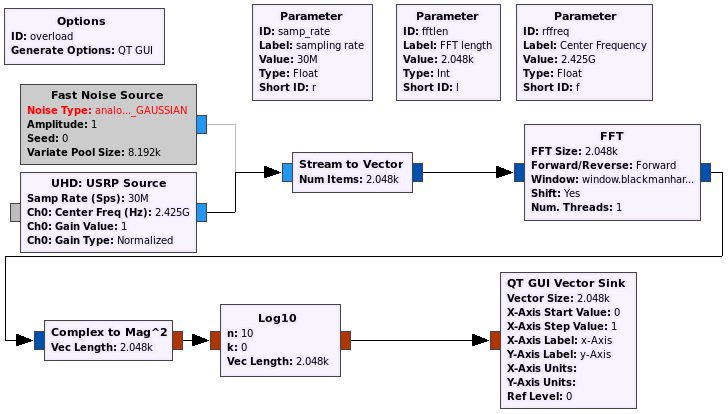
\includegraphics[height=0.75\textheight]{overload}}
\end{frame}

\end{document}
